\chapter{Task 6}
\begin{figure}[hbt]	
\label{Task6}
  \centering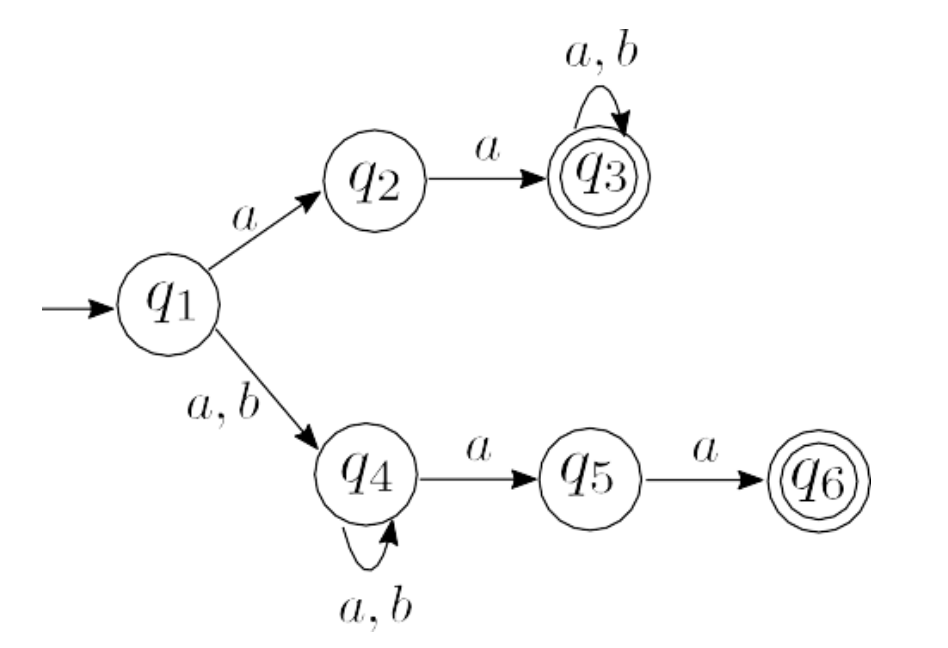
\includegraphics[width=0.9\textwidth]{Immagini/fsm_task6.png}
  \caption{Task6}
\end{figure}
The Figure shown above, represent a NFA that accepts the language composed by the alphabet ${a,b, \epsilon}$ where all strings accepted are the ones that contain the substring: "$aa$".

The reason being the fact that NFA when given an input that would be processed by multiple state, like in this case the input $a$ would be accepted simultaneously by state $q_2$ and $q_4$; the machine would be split up in two different machine and if even one of the multiple machine in which an NFA would split accept the given input then, the input is accepted.